\section{Results}
\label{sec:results}
The results follow the endpoints: first the decomposition of the damage per ratio, then the acceleration, the classes on which each factor's damage lands, the effect of logit adjustment, and finally the selected regularization and temperatures. The balanced arm reaches 39.57 percent balanced accuracy (36.70 to 42.53), as in the prevalence curve.

\subsection{Decomposition of the damage}
\label{sec:decomposition-results}
Both factors cost accuracy on BRACS, and their damages add up to nearly the full damage at every ratio (Table~\ref{tab:decomposition}, Figure~\ref{fig:component}). The prior alone accounts for the larger part: 1.02 of the 1.15 points at $\rho=2$, 2.79 of 3.86 points at $\rho=10$, and 4.37 of 7.98 points at $\rho=100$. Its intervals lie clearly above zero from $\rho=5$ on; at $\rho=2$ the lower bound is close to zero. Unlike on TCGA-UT, where thin support alone cost nothing up to $\rho=20$ \citep{queisler2026causeTcga}, the support-only damage on BRACS is resolved from $\rho=10$ on, 0.87 points at $\rho=10$, where the tail class keeps 7.7 patches per patient, and it grows to 3.30 points at $\rho=100$, where the tail keeps 1.2. A balanced objective on the long-tailed rows thus does not protect the BRACS classifier once the tail falls below about eight patches per patient.

\begin{table}[htbp]
\centering
\small
\setlength{\tabcolsep}{4pt}
\renewcommand{\arraystretch}{1.15}
\begin{tabular}{@{}lllllrr@{}}
\toprule
$\rho$ & $\Delta_\text{r}$ (both) & $\Delta_\text{P}$ (prior) & $\Delta_\text{S}$ (support) & Interaction $I$ & Share P & Share S \\
\midrule
2 & 1.15 [0.14, 2.35] & 1.02 [0.05, 2.19] & 0.11 [$-$0.36, 0.59] & 0.03 [$-$0.55, 0.60] & 0.88 & 0.10 \\
5 & 2.97 [1.62, 4.46] & 2.22 [0.96, 3.57] & 0.58 [$-$0.06, 1.32] & 0.18 [$-$0.74, 0.96] & 0.74 & 0.20 \\
10 & 3.86 [2.33, 5.44] & 2.79 [1.39, 4.29] & 0.87 [0.07, 1.74] & 0.20 [$-$0.72, 0.996] & 0.72 & 0.23 \\
20 & 5.08 [3.34, 6.94] & 3.71 [2.11, 5.36] & 1.37 [0.49, 2.30] & 0.01 [$-$1.17, 1.02] & 0.73 & 0.27 \\
50 & 6.60 [4.76, 8.65] & 3.96 [2.40, 5.58] & 2.24 [1.18, 3.39] & 0.40 [$-$0.90, 1.56] & 0.60 & 0.34 \\
100 & 7.98 [6.01, 10.17] & 4.37 [2.77, 5.99] & 3.30 [1.99, 4.68] & 0.31 [$-$1.28, 1.71] & 0.55 & 0.41 \\
\bottomrule
\end{tabular}
\caption{On BRACS the prior carries the larger part of the damage, thin support the rest, and their sum is close to the full damage at every ratio. Damages are balanced-accuracy losses against the balanced arm in percentage points, with paired 95\% bootstrap intervals; the interaction is $\Delta_\text{r}-\Delta_\text{P}-\Delta_\text{S}$. Shares are single-factor damages as fractions of $\Delta_\text{r}$. Their intervals at $\rho=100$ are 0.42 to 0.68 for P and 0.28 to 0.55 for S; at $\rho=2$ they span 0.29 to 1.54 and $-0.80$ to 0.56.}
\label{tab:decomposition}
\end{table}

\noindent No interaction is detected. Its point estimates lie between 0.01 and 0.40 points at all six ratios, and $\Delta_\text{P}+\Delta_\text{S}$ at $\rho=100$ is 7.67 points against a full damage of 7.98. Every interval contains zero. Up to $\rho=10$ the intervals also stay within $\pm1$ point, the one at $\rho=10$ only just, with an upper bound of 0.996; from $\rho=20$ on they reach 1.02 to 1.71 points. By the criterion fixed in Section~\ref{sec:evaluation}, the factors are additive from $\rho=2$ to 10, and the interaction is unresolved at the larger ratios. The upper bound at $\rho=100$, 1.71 points, is 21 percent of the full damage, about half of the 43 percent that the interaction contributes on TCGA-UT \citep{queisler2026causeTcga}. The shares move with $\rho$: the prior carries 72 to 74 percent of the damage from $\rho=5$ to 20 and 55 percent at $\rho=100$, while the support share rises from 0.10 at $\rho=2$ to 0.41. No split shows compounding of the size found on TCGA-UT; the interactions at $\rho=100$ are 0.14, 0.32, and 0.45 points.

\begin{figure}[htbp]
\centering
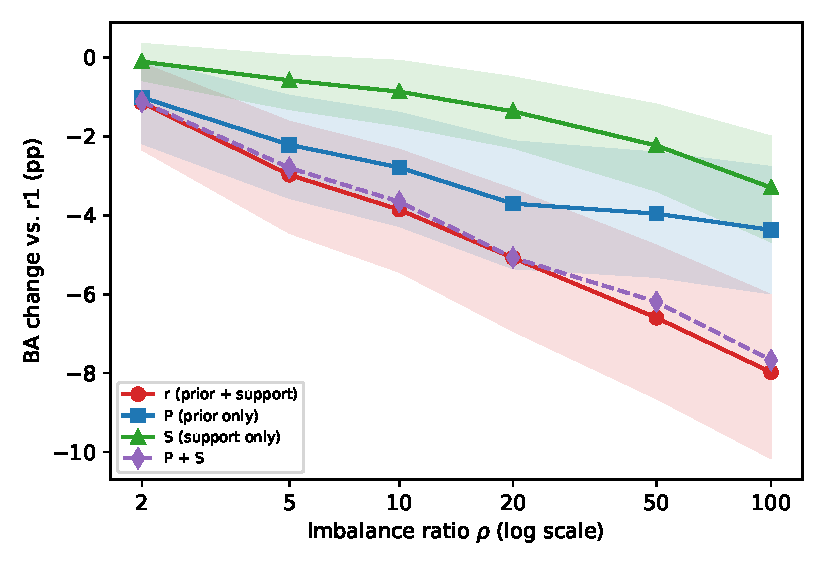
\includegraphics[width=0.6\textwidth]{component.pdf}
\caption{On BRACS the full damage is close to the sum of its single-factor parts. Change in patient-macro balanced accuracy relative to the balanced arm for the ratio arm r (prior and support), the prior-only arm P, and the support-only arm S, each with a shaded paired 95\% bootstrap band; the dashed line is the sum of the P and S changes. All series are plotted at the realized ratio of r$\rho$.}
\label{fig:component}
\end{figure}

\subsection{Acceleration}
\label{sec:acceleration-results}
No family accelerates, but the two factors change their rates in opposite directions (Table~\ref{tab:slopes}). The full damage grows by 1.19 points per doubling of $\rho$ up to $\rho=10$ and by 1.23 points beyond, so its acceleration of 0.04 points is not resolved, as in the prevalence curve. The prior-only damage grows faster at low ratios, 0.77 points per doubling, than at high ratios, 0.44 points. The support-only damage does the opposite, 0.33 points per doubling up to $\rho=10$ and 0.72 points beyond. Neither slope difference is resolved, although the support family comes close with an interval of $-0.04$ to 0.80 points. Below $\rho=10$ the prior thus contributes about 65 percent of the growth; above it, support contributes about 60 percent, and the two changes offset each other in the nearly linear full curve.

\begin{table}[htbp]
\centering
\renewcommand{\arraystretch}{1.15}
\begin{tabular}{@{}llll@{}}
\toprule
Family & Slope, $\rho\leq10$ & Slope, $\rho\geq10$ & Acceleration \\
\midrule
r (both) & 1.19 [0.74, 1.65] & 1.23 [0.89, 1.64] & 0.04 [$-$0.50, 0.56] \\
P (prior) & 0.77 [0.36, 1.24] & 0.44 [0.24, 0.63] & $-$0.33 [$-$0.86, 0.14] \\
S (support) & 0.33 [0.04, 0.67] & 0.72 [0.44, 1.04] & 0.39 [$-$0.04, 0.80] \\
\bottomrule
\end{tabular}
\caption{The prior damage grows fastest at low ratios and the support damage at high ratios, while the full damage grows at a constant rate. Least-squares slopes of the damage on $\log_2\rho$ in points per doubling, with paired 95\% bootstrap intervals; acceleration is the high-segment slope minus the low-segment slope. None is resolved above zero. The low segment of r includes the balanced arm at $\rho=1$; those of P and S start at $\rho=2$.}
\label{tab:slopes}
\end{table}

\subsection{Where the damage lands}
\label{sec:rank-results}
Both factors move recall from the tail and body classes to the head classes, and at $\rho=100$ they do so with similar strength (Table~\ref{tab:thirds}). The prior-only arm removes most of its tail recall at small ratios: tail recall falls from 38.73 percent in the balanced arm to 27.87 at $\rho=2$ and to 20.75 at $\rho=10$, and then stays between 20.3 and 20.8 percent up to $\rho=100$. Its head gain peaks at 9.5 points at $\rho=10$ and shrinks to 6.8 points at $\rho=100$. The support-only arm leaves the head within 4.5 points of the balanced arm up to $\rho=20$ but loses tail recall steadily, from 36.86 percent at $\rho=2$ to 19.36 at $\rho=100$. At $\rho=100$ it lowers the tail by 19.4 points and raises the head by 7.8, more than the prior-only arm does on either group, although its objective is balanced.

\begin{table}[htbp]
\centering
\small
\renewcommand{\arraystretch}{1.15}
\begin{tabular}{@{}lrrrrrrrrrr@{}}
\toprule
 & & \multicolumn{3}{c}{$\rho=10$} & \multicolumn{3}{c}{$\rho=20$} & \multicolumn{3}{c}{$\rho=100$} \\
\cmidrule(lr){3-5}\cmidrule(lr){6-8}\cmidrule(lr){9-11}
Group & r1 & r & P & S & r & P & S & r & P & S \\
\midrule
Head (3) & 37.41 & 50.01 & 46.89 & 40.96 & 50.36 & 45.33 & 41.84 & 52.36 & 44.17 & 45.22 \\
Body (2) & 43.66 & 34.48 & 37.65 & 41.85 & 32.94 & 36.74 & 41.23 & 26.00 & 36.67 & 39.76 \\
Tail (2) & 38.73 & 15.50 & 20.75 & 32.16 & 12.23 & 20.79 & 29.71 & 6.04 & 20.27 & 19.36 \\
\bottomrule
\end{tabular}
\caption{At $\rho=100$ the thin support costs the tail as much as the skewed prior, and the ratio arm loses less tail recall than the two factors together but more body recall. Mean patient-macro recall in percent of the three head, two body, and two tail classes of each draw, by their assigned rank, averaged over 30 fits. The r columns are taken from the prevalence curve.}
\label{tab:thirds}
\end{table}

\noindent Within the rank groups, the factors do not add up, even though they nearly do in balanced accuracy. At $\rho=100$ the tail loss of the ratio arm, 32.7 points, is 5.1 points smaller than the sum of the single-factor tail losses, 37.8 points, which would leave the tail classes with only 0.9 percent recall. The body loss of the ratio arm, 17.7 points, exceeds the single-factor sum of 10.9 points by 6.8 points, and the head gains are close to additive, 15.0 against 14.6 points. Because two classes each form the body and the tail, the two deviations largely cancel in balanced accuracy, and what remains is the interaction of 0.31 points. A floor effect in the tail is the simplest explanation: once the tail classes are hardly predicted at all, a further push cannot remove more of their recall, and the combined push lands on the next ranks instead.

\subsection{Logit adjustment}
\label{sec:adjustment-results}
Post-hoc logit adjustment repairs a third of the ratio arm's damage and leaves the prior-only arm nearly unchanged (Table~\ref{tab:adjustment}). Applied to r100, it raises balanced accuracy from 31.59 to 34.16 percent, a recovery of 2.56 of the 7.98 points, and at $\rho=10$ it recovers 1.57 of 3.86 points. It falls 2.11 points (1.00 to 3.35) short of the support-only arm, which trains on the same rows with a balanced objective, and it falls short of it at every ratio from $\rho=5$ on, by 1.16 to 2.37 points. Applied to P$\rho$, the same correction raises balanced accuracy by between 0.04 and 0.72 points, but the intercept share of the prior damage is not resolved at any ratio: it is 0.26 ($-0.19$ to 0.55) at $\rho=10$ and 0.02 ($-0.31$ to 0.25) at $\rho=100$. On TCGA-UT, the same correction lowered the prior-only arm by 0.57 points at $\rho=100$ \citep{queisler2026causeTcga}; on BRACS it has no resolved effect. In both datasets the weighted fit has therefore not shifted its class intercepts by the log prior, and its damage lies elsewhere in the fitted scores.

\begin{table}[htbp]
\centering
\renewcommand{\arraystretch}{1.15}
\begin{tabular}{@{}lrrrrrl@{}}
\toprule
$\rho$ & r & Lr & P & LP & S & Lr $-$ S \\
\midrule
10 & 35.71 & 37.28 & 36.78 & 37.50 & 38.70 & $-$1.42 [$-$2.43, $-$0.38] \\
20 & 34.49 & 36.46 & 35.86 & 36.33 & 38.20 & $-$1.74 [$-$2.88, $-$0.60] \\
50 & 32.97 & 34.96 & 35.61 & 35.65 & 37.33 & $-$2.37 [$-$3.54, $-$1.26] \\
100 & 31.59 & 34.16 & 35.20 & 35.29 & 36.27 & $-$2.11 [$-$3.35, $-$1.00] \\
\bottomrule
\end{tabular}
\caption{Logit adjustment helps the ratio arm but stays well below training-time rebalancing, and it leaves the prior-only arm nearly unchanged. Test patient-macro balanced accuracy in percent; the balanced arm reaches 39.57. Lr and LP subtract the log training prior from the logits of r and P; the last column is the paired difference between post-hoc and training-time correction of the same rows, with its 95\% bootstrap interval.}
\label{tab:adjustment}
\end{table}

\subsection{Regularization and temperature}
\label{sec:selection-results}
The prevalence curve found that stronger imbalance selects much weaker regularization and a much larger temperature on BRACS: the balanced arm selects $\lambda=1$ or 10 in all 30 fits with a mean temperature of 0.65, whereas r100 selects $\lambda\leq10^{-3}$ in 11 fits and reaches a temperature of 4.43 \citep{queisler2026prevalenceBracs}. As on TCGA-UT, the prior causes most of this shift. The support-only arms select $\lambda=1$ or 10 in 27 to 29 of 30 fits at every ratio, like the balanced arm, and their mean temperature rises only from 0.66 at $\rho=2$ to 0.91 at $\rho=100$. The prior-only arms move toward weaker regularization as $\rho$ grows: $\lambda=1$ in 23 of 30 fits at $\rho=2$, $\lambda=0.1$ in 20 at $\rho=10$, and $\lambda\leq10^{-2}$ in 24 at $\rho=100$, 15 of them at $\lambda\leq10^{-3}$. Their mean temperature rises from 0.89 at $\rho=2$ to 4.04 at $\rho=100$, well above the balanced arm and close to the 4.43 of r100.

The prior-only arms reach the smallest grid value, $10^{-6}$, in 2 fits at $\rho=20$, 1 at $\rho=50$, and 5 at $\rho=100$; the support-only arms never do, but one support-only fit at $\rho=10$ selects the largest value, 100. When the eight boundary fits of the prior-only arms are refitted with $\lambda$ extended down to $10^{-10}$, validation selects a smaller value in all eight, with gains of 0.09 to 1.17 points of validation balanced accuracy. Selection on the extended grid changes the test balanced accuracy of these fits by $-0.99$ to 1.94 points, and the damage by at most 0.05 points at any ratio. Extended up to $10^{4}$, the grid confirms $\lambda=100$ for the support-only fit, with 40.21 percent validation balanced accuracy against 39.63 at $10^{3}$. The grid boundary therefore does not affect the results.

\section{Discussion}
\label{sec:discussion}
Of the readings fixed in Section~\ref{sec:evaluation}, none of the directional ones applies at $\rho=100$. The prior-only damage of 4.37 points exceeds one point and carries 55 percent of the full damage, but the support-only damage of 3.30 points also exceeds one point, so the prior does not carry the damage in the pre-stated sense, and support does not either. The interaction is not resolved above zero; its point estimate of 0.31 points is small, but its interval is too wide to meet the additive criterion. No family shows a resolved acceleration, so none is attributed. The data thus describe two single factors of comparable order, the prior the larger one, whose damages add up in balanced accuracy to within the precision of the study.

The explanation proposed by the prevalence study holds only in part. Its first half is supported: the skewed prior is the larger factor at every ratio, and on its own, with 320 patches in every class, it costs 4.37 points at $\rho=100$, 4.2 times the 1.04 points of the same arm on TCGA-UT \citep{queisler2026causeTcga}. A prior-only arm keeps the tail fully supported, so this damage cannot come from thin support, and its size fits the proposed mechanism that overlapping lesion classes let a skewed prior shift the decision boundaries far into the rare classes. The prior-only arm also removes most of its tail recall already at $\rho=2$ to 10, as the BRACS curve did. The second half, that thin tail support does not matter, is refuted. A balanced objective on the long-tailed rows costs 0.87 points at $\rho=10$ and 3.30 points at $\rho=100$, more than the whole prevalence damage on TCGA-UT. At $\rho=10$ the tail classes of both datasets keep about eight patches per patient, yet support alone costs 0.87 points on BRACS and nothing on TCGA-UT. BRACS classes are thus harder to estimate from few patches as well as more sensitive to the prior, which is consistent with overlap acting on both factors. The steeper profile of seven classes adds to the support effect, because the tail class receives 12 of 2,240 patches at $\rho=100$ and its weight in the support-only arm rises to 26.7.

The comparison with TCGA-UT is summarized in Table~\ref{tab:cross}. The two datasets differ less in which factor dominates than in how the factors combine. On TCGA-UT, the prior dominates at moderate ratios and the two factors compound at large ratios, with an interaction larger than the prior damage. On BRACS, both factors cost accuracy from moderate ratios on and no compounding is detected. The rank-group recall suggests why: on BRACS the prior alone already reduces the tail classes to about 20 percent recall, and the combination cannot push them much further, so the extra loss appears in the body classes and largely cancels in balanced accuracy. On TCGA-UT the tail third keeps 60 percent recall even at $\rho=100$, so the combined push can still lower it. Whether the BRACS interaction is truly small or only hidden by this floor cannot be decided from balanced accuracy alone.

\begin{table}[htbp]
\centering
\renewcommand{\arraystretch}{1.15}
\begin{tabular}{@{}lrrrrrrr@{}}
\toprule
Dataset, $\rho$ & $\Delta_\text{r}$ & $\Delta_\text{P}$ & $\Delta_\text{S}$ & $I$ & Share P & Share S & Lr $-$ S \\
\midrule
TCGA-UT, 10 & 0.57 & 0.49 & $-$0.05 & \textbf{0.14} & --- & --- & $-$0.31 \\
BRACS, 10 & 3.86 & 2.79 & 0.87 & 0.20 & 0.72 & 0.23 & $-$1.42 \\
\addlinespace
TCGA-UT, 100 & 2.76 & 1.04 & 0.54 & \textbf{1.18} & 0.38 & 0.19 & $-$0.73 \\
BRACS, 100 & 7.98 & 4.37 & 3.30 & 0.31 & 0.55 & 0.41 & $-$2.11 \\
\bottomrule
\end{tabular}
\caption{Both factors are larger on BRACS, but only TCGA-UT shows a resolved interaction. Damages and interaction in percentage points against each dataset's balanced arm, in bold where the interaction is resolved above zero; the last column is the balanced-accuracy gap between logit-adjusted ratio arm and support-only arm. TCGA-UT values are taken from \citet{queisler2026causeTcga}; its shares at $\rho=10$ are omitted because its full damage lies below one point.}
\label{tab:cross}
\end{table}

\noindent For mitigation, the decomposition points to training-time rebalancing, as on TCGA-UT, and it also shows its limit on BRACS. Restoring a balanced objective on the rows of r$\rho$ removes the prior damage and leaves the support-only damage, 3.30 points at $\rho=100$. Post-hoc logit adjustment of the same classifier recovers only a third of the full damage and stays 2.11 points below that level. The remaining support-only damage is not small on BRACS: it exceeds the prevalence damage at $\rho=5$, so rebalancing alone cannot restore a long-tailed BRACS training set, and more tail patches or patients would be needed.

\section{Limitations}
\label{sec:limitations}
The prior-only arm imposes the long-tailed prior by class weights, not by resampling, and the support-only arm restores the balanced prior the same way. The weighted objectives have the right expectation but are not the same estimators as sampled ones: at $\rho=100$ the support-only arm gives each of the twelve tail patches a weight of 26.7, which may let a regularized classifier overfit them, and the head rows of the prior-only arm number 320 rather than 1,206. The support-only damage therefore mixes the effect of thin support with any cost of extreme weights, and the interaction mixes compounding with any difference between weighting and sampling. Each fitted arm selects its own regularization, so the decomposition includes the effect of the prior on model selection.

The rank groups contain three, two, and two classes, so the body and tail recall of Table~\ref{tab:thirds} rest on two classes per draw and mix the imbalance effect with the difficulty of the classes that drew each rank; the floor argument for the small interaction relies on these groups. With about 24 test patients per split, the intervals of the interaction are about three times wider than on TCGA-UT and cannot exclude an interaction of one point. The low-segment slopes of P and S are estimated from three ratios. All results are conditional on ten patients per class, frozen Virchow2 features, multinomial logistic regression, BRACS, and three overlapping splits.
